%% LyX 1.3 created this file.  For more info, see http://www.lyx.org/.
%% Do not edit unless you really know what you are doing.
\documentclass[english, 12pt]{article}
\usepackage{times}
%\usepackage{algorithm2e}
\usepackage{url}
\usepackage{bbm}
\usepackage[T1]{fontenc}
\usepackage[latin1]{inputenc}
\usepackage{geometry}
\geometry{verbose,letterpaper,tmargin=2.5cm,bmargin=2.5cm,lmargin=2.5cm,rmargin=2.5cm}
\usepackage{rotating}
\usepackage{color}
\usepackage{graphicx}
\usepackage{subcaption}
\usepackage{amsmath, amsthm, amssymb}
\usepackage{setspace}
\usepackage{lineno}
\usepackage{hyperref}
\usepackage{bbm}


%\usepackage{xr}
%\externaldocument{SCT-supp}

\linenumbers
\doublespacing
%\usepackage[authoryear]{natbib}
\usepackage{natbib} \bibpunct{(}{)}{;}{author-year}{}{,}

%Pour les rajouts
\usepackage{color}
\definecolor{trustcolor}{rgb}{0,0,1}

\usepackage{dsfont}
\usepackage[warn]{textcomp}
\usepackage{adjustbox}
\usepackage{multirow}
\usepackage{graphicx}
\graphicspath{{../figures/}}
\DeclareMathOperator*{\argmin}{\arg\!\min}

\let\tabbeg\tabular
\let\tabend\endtabular
\renewenvironment{tabular}{\begin{adjustbox}{max width=0.9\textwidth}\tabbeg}{\tabend\end{adjustbox}}

\makeatletter

%%%%%%%%%%%%%%%%%%%%%%%%%%%%%% LyX specific LaTeX commands.
%% Bold symbol macro for standard LaTeX users
%\newcommand{\boldsymbol}[1]{\mbox{\boldmath $#1$}}

%% Because html converters don't know tabularnewline
\providecommand{\tabularnewline}{\\}

\usepackage{babel}
\makeatother


\begin{document}


\title{Making the most out of Clumping and Thresholding}
\author{Florian Priv\'e,$^{\text{1,}*}$ Bjarni J. Vilhj\'almsson,$^{\text{2}}$ Hugues Aschard$^{\text{3}}$ and Michael G.B. Blum$^{\text{1,}*}$}



\date{~ }
\maketitle

\noindent$^{\text{\sf 1}}$Laboratoire TIMC-IMAG, UMR 5525, Univ.\ Grenoble Alpes, CNRS, La Tronche, France, \\
\noindent$^{\text{\sf 2}}$National Center for Register-based Research, Aarhus University, Denmark. \\
\noindent$^{\text{\sf 3}}$Centre de Bioinformatique, Biostatistique et Biologie Int\'egrative (C3BI), Institut Pasteur, Paris, France,

\noindent$^\ast$To whom correspondence should be addressed.\\

\noindent Contacts:
\begin{itemize}
\item \url{florian.prive@univ-grenoble-alpes.fr}
\item \url{bjv@econ.au.dk}
\item \url{hugues.aschard@pasteur.fr}
\item \url{michael.blum@univ-grenoble-alpes.fr}
\end{itemize}

\newpage

\abstract{

}


%%%%%%%%%%%%%%%%%%%%%%%%%%%%%%%%%%%%%%%%%%%%%%%%%%%%%%%%%%%%%%%%%%%%%%%%%%%%%%%%

\newpage

\section{Introduction}

Clumping and Thresholding (C+T, also called P+T) is a simple technique for computing Polygenic Risk Scores (PRS) based on Genome-Wide Association Studies (GWAS) summary statistics, and has been used for more than ten years \cite[]{euesden2014prsice,purcell2009common}.
C+T consists in making a simple sum of allele counts (genotypes), weighted by effect sizes from GWAS summary statistics, after having restricted the variants included in this sum, twice.
The SNPs are first clumped (C) so that there remains only SNPs that are weakly correlated with each other ($S_{\text{clumping}}$). Clumping looks at the most significant SNP first, computes correlation between this index SNP and nearby SNPs (within some genetic distance $w_c$) and remove all the nearby SNPs that are correlated with this index SNP beyond a particular threshold $r_{c}^2$. 
The clumping step aims at removing redundancy in included effects that is simply due to linkage disequilibrium (LD) between variants. Yet, this procedure may as well remove independently predictive variants in nearby regions.
Thresholding (T) consists in removing SNPs that are under a chosen level of significance ($p > p_T$), which aims at reducing noise in the score.

When applying C+T, one has to choose at least 3 hyper-parameters: for clumping, the squared correlation threshold $r_{c}^2$ and the window size $w_c$ of clumping [RENAME?? e.g.\ $d_c$]; for thresholding, the p-value threshold $p_T$.
More often than otherwise, C+T users fix default values for clumping, such as $r_{c}^2$ of 0.1 (default of PRSice), 0.2  or 0.5 (default of PLINK), and $w_c$ of 250kb (default of PRSice and PLINK) or 500kb, and test values for $p_T$ ranging from $1$ to $10^{-8}$ at most \cite[]{wray2014research,euesden2014prsice,chang2015second}.
Moreover, to match the variants of the GWAS summary statistics, one need to use imputed data to get the same variants in the data to compute the PRS on. 
A liberal inclusion of variants is often accepted, with the assumption that the more variants there are in the model, the better would be the prediction, whatever the imputation accuracy of these variants. 
Here, we consider this threshold on quality of imputation (often called the INFO score) as a fourth parameter of the C+T method.

Here, we show that these four hyper-parameters are really important, and that choosing those hyper-parameters well could substantially increase the predictive power of C+T over using current default parameters.
We implement an efficient way to compute C+T scores for many different parameters in R package bigsnpr \cite[]{prive2017efficient}. 
Moreover, instead of choosing the set of parameters that corresponds to the best prediction, we use stacking, i.e.\ we learn an optimal combination of all C+T scores to improve prediction beyond the best prediction of any of these scores \cite[]{breiman1996stacked}.
We call this method SCT, which stands for Stacked Clumping and Thresholding.
Using the UK Biobank data \cite[]{bycroft2017genome} and external summary statistics for simulated and real data analyses, we show that testing a larger grid of parameters consistently improves predictions as compared to using some default parameters for C+T. We also show that SCT consistently improves predictions over any single C+T prediction.

%%%%%%%%%%%%%%%%%%%%%%%%%%%%%%%%%%%%%%%%%%%%%%%%%%%%%%%%%%%%%%%%%%%%%%%%%%%%%%%%

\section{Material and Methods}

\subsection{Simulations}

We use variants from the UK Biobank (UKBB) imputed dataset that have a minor allele frequency larger than 1\% and an imputation INFO score larger than 0.3. There are almost 10M such variants, we randomly choose 1M of them.
To limit population structure and family structure, we restrict individuals to the ones referred as of White British ancestry by the UK Biobank and exclude all second individuals in each pair reported as related individuals by the UK Biobank \cite[]{bycroft2017genome}.
335,609 individuals remain and we split them in three sets: one for training (e.g.\ choosing the hyper-parameters) and one for testing (evaluating the models) for which we sample 10,000 different individuals in both sets; and one for computing summary statistics (GWAS) with the 315,609 remaining individuals.

For simulating phenotypes and computing summary statistics, we transform UKBB data into hard calls by randomly sampling hard calls according to imputation probabilities.
For the train and test sets, we transform these probabilities in dosage (expected) values. 
We are able to read from UKBB BGEN files using function \texttt{snp\_readBGEN} of package bigsnpr \cite[]{prive2017efficient}.
This enables us to simulate phenotypes using ``real'' underlying genotypes as hard calls and use the INFO score (imputation accuracies) reported by the UK Biobank to assess the quality of the imputed data. [END CLEAR ENOUGH??]

We simulate binary phenotypes with a heritability $h^2 = 0.5$ using a Liability Threshold Model (LTM) with a prevalence of 10\% \cite[]{falconer1965inheritance}. We vary the number of causal variants (100, 10K, or 1M) in order to match a range of genetic architectures from low to high polygenicity.
Liability scores are computed from a model with additive effects only: we compute the liability score of the i-th individual as \(y_i = \sum_{j\in S_\text{causal}} w_j \widetilde{G_{i,j}} + \epsilon_i,\) where $S_\text{causal}$ is the set of causal SNPs, $w_j$ are weights generated from a Gaussian distribution $N(0, h^2 / \vert S_\text{causal} \vert)$, $G_{i,j}$ is the allele count of individual $i$ for SNP $j$, $\widetilde{G_{i,j}}$ corresponds to its standardized version (zero mean and unit variance for all SNPs), and $\epsilon$ follows a Gaussian distribution $N(0, 1 - h^2)$.
We also add three more complex architectures: ``2chr'', 100 SNPs of chromosome 1 and all SNPs of chromosome 2 are causal, with half of the heritability for both chromosomes; ``err'', we sample 10,000 random causal SNPs, but 10\% of the GWAS effects are reported with an opposite effect; ``HLA'', 7105 causal SNPs are chosen in one long-range LD region of chromosome 6.

To compute summary statistics, we use Cochran-Armitage additive test \cite[]{zheng2012analysis}. Given that we restricted the data to have minimal population structure, this test based on contingency tables is much faster than using a logistic regression with 10 principal components as covariates (40 minutes vs 16 hours) while providing similar effect sizes and Z-scores (Figure \ref{fig:GWAS}).

Each simulation is repeated 10 times.

\subsection{Real summary statistics}

We also investigate prediction using real summary statistics from published GWAS, summarized in table \ref{tab:sumstats} \cite[]{buniello2018nhgri}.
As in simulations, we restrict individuals to the ones referred as of White British ancestry by the UK Biobank and exclude all second individuals in each pair reported as related individuals by the UK Biobank \cite[]{bycroft2017genome}.
As some reproducible code is worth a thousand words, we invite the reader to look at our analysis code to see how we define phenotypes in the UK Biobank; we summarize the number of cases and controls for each phenotype in table \ref{tab:sumstats}.

\begin{table}[h]
\caption{Available cases and controls in UK Biobank (UKBB) for many binary traits, along with corresponding published GWAS summary statistics. Summary statistics are chosen from GWAS that did not include individuals from UKBB. For depression, we remove UKBB individuals from the pilot release since they were included in the GWAS we use here.\label{tab:sumstats}}
\vspace*{0.5em}
\centering
\begin{tabular}{|l|c|c|c|c|c|}
  \hline
Trait & UKBB size & GWAS size & GWAS \#SNPs & GWAS citation \\
  \hline
Breast cancer (BRCA) & ~~11,578 / 158,391 & 137,045 / 119,078 & 11,792,542 & \cite{michailidou2017association} \\
Rheumatoid arthritis (RA) & ~~~~~5615 / 226,327 & ~~29,880 / ~~73,758 & ~~9,739,303 & \cite{okada2014genetics} \\
Type 1 diabetes (T1D) & ~~~~~~~771 / 314,547 & ~~~~~5913 / ~~~~~8828  & ~~8,996,866 & \cite{censin2017childhood} \\
Type 2 diabetes (T2D) & ~~14,176 / 314,547 & ~~26,676 / 132,532 & 12,056,346 & \cite{scott2017expanded} \\
Prostate cancer (PRCA) & ~~~~~6643 / 141,321 & ~~79,148 / ~~61,106 & 20,370,946 & \cite{schumacher2018association} \\
Depression (MDD) & ~~26,134 / 291,690 & ~~59,851 / 113,154 & 13,554,550 & \cite{wray2018genome} \\
Coronary artery disease (CAD) & ~~12,263 / 225,927 & ~~60,801 / 123,504 & ~~9,455,778 & \cite{nikpay2015comprehensive} \\
Asthma & ~~43,787 / 261,985 & ~~19,954 / 107,715 & ~~2,001,280 & \cite{demenais2018multiancestry} \\
  \hline
\end{tabular}
\end{table}

We keep all variants with a GWAS p-value lower than 0.1. 
To match remaining summary statistics with data from the UK Biobank, we first remove ambiguous alleles [A/T] and [C/G]. We then augment the summary statistics twice: first by adding copied rows with the complementary alleles, then by adding copied rows with reverse alleles and effects. Finally, we use an inner join on the combination of chromosome, position and the two alleles to match these augmented summary statistics with data from the UK Biobank. Note that, when there are no or very few alleles that are flipped, we disable the strand flipping option and therefore do not remove ambiguous alleles.

\subsection{Clumping and Thresholding (C+T) and Stacked C+T (SCT)}

We compute C+T scores \textit{for each chromosome separately} and for many parameters:
\begin{itemize}
\item Threshold on imputation INFO score within \{0.3, 0.6, 0.9, 0.95\}.
\item Squared correlation threshold of clumping $r_{c}^2$ within \{0.01, 0.05, 0.1, 0.2, 0.5, 0.8, 0.95\}.
\item Base size of clumping window within \{50, 100, 200, 500\}. $w_c$ is then computed as the base size divided by $r_{c}^2$. For example, for $r_{c}^2 = 0.2$, we test values of $w_c$ within \{250, 500, 1000, 2500\} (in kb). This is motivated by the fact that linkage disequilibrium is inversely proportional to genetic distance between variants \cite[]{pritchard2001linkage}.
\item A sequence of 50 thresholds on p-values between 0.1 (-log10(p) = 1) and the most significant p-value, equally spaced on a log-log scale.
\end{itemize}
Thus, for individual $i$, chromosome $k$ and the four hyper-parameters info\_thr, $r_{c}^2$, $w_c$ and $p_T$, we compute
\[\rm{V}_i^{(k)}(\text{info\_thr},~r_{c}^2,~w_c,~p_T) = \sum_{\substack{j ~\in~ \text{chromosome k} \\ \text{INFO}_j ~\geq~ \text{info\_thr} \\ j ~\in~ S_\text{clumping}(r_{c}^2,~w_c) \\ p_j~<~p_T}} \hat\beta_j \cdot G_{i,j}~,\] where $\hat\beta_j$ ($p_j$) are the effect sizes (p-values) estimated from the GWAS and $G_{i,j}$ is the dosage for individual $i$ and SNP $j$.
%Computation time is largely driven by the computation of clumping sets, which consists mainly in computing squared correlations between pairs of variants. So, to speed-up the overall computation, we cache the computation of those correlations.

Overall, we compute $22 \times 4 \times 7 \times 4 \times 50 = 123200$ vectors of polygenic scores.
Then, we stack all these polygenic scores (for individuals in the training set) by using these scores as variables in an efficient penalized logistic regression available in our R package bigstatsr \cite[]{prive2019efficient}.
This results in a linear combination of C+T scores from which we derive a single vector of  effect sizes. The resulting single vector of new effect sizes is used for evaluation in the test set. 
We refer to this method as ``SCT'' in the rest of the paper.

From this grid, we derive two C+T scores: one using some default parameters, i.e.\ with $r_{c}^2$ = 0.2, $w_c$ = 500, a liberal threshold of 0.3 on imputation INFO score, and choosing the p-value threshold (between $0.1$ and $10^{-8}$) maximizing the AUC on the training set; one corresponding to the set of the previous four parameters that maximizes AUC on the training set. 
We refer to these methods as ``stdCT'' and ``maxCT'' in the rest of the paper.
Note that stdCT and maxCT use the same set of parameters for all chromosomes, i.e.\ for one set of the four hyper-parameters, they are defined as $\rm{V}^{(1)} + \cdots + \rm{V}^{(22)}$.

%%%%%%%%%%%%%%%%%%%%%%%%%%%%%%%%%%%%%%%%%%%%%%%%%%%%%%%%%%%%%%%%%%%%%%%%%%%%%%%%

\section{Results}

\subsection{Simulations}

We test 6 different simulations scenarios. 
In all these scenarios, maxCT --that tests a much larger grid of hyper-parameters values for C+T on the training set-- consistently provides higher AUC values on the test set as compared to stdCT that tests only a limited  of hyper-parameters values. 
The absolute improvement in AUC of maxCT over stdCT is particularly large in the cases of 100 and 10,000 causal SNPs, where causal effects are mostly independent of one another. 
In these cases, using a very stringent $r_{c}^2 = 0.01$ threshold of clumping provides higher predictive performance than using a standard default of $r_{c}^2 = 0.2$ (Figures \ref{fig:simugridA} and \ref{fig:simugridB}). However, $r_{c}^2 = 0.2$ seems to be an appropriate default when simulating 1M causal variants, but still the default window size is not large enough and an increasing window size increases AUC (Figure \ref{fig:simugridC}).

As for SCT, it provides equal or higher predictive performance than maxCT in simulation scenarios. In the first three simple scenarios simulating 100, 10K or 1M causal SNPs anywhere on the genome, predictive performance of SCT are similar to maxCT. In the ``2chr'' scenario where there are large effects on chromosome 1, smaller effects on chromosome 2 and no effect on other chromosomes, mean AUC is 0.787 for maxCT and 0.822 for SCT, which is an absolute increase of 4.5\%. In the ``err'' scenario where we report GWAS summary statistics with 10\% reversed effects (errors), mean AUC is 0.702 for maxCT and 0.732 for SCT, which is an absolute increase of 3\%.


\begin{figure}[h]
\centerline{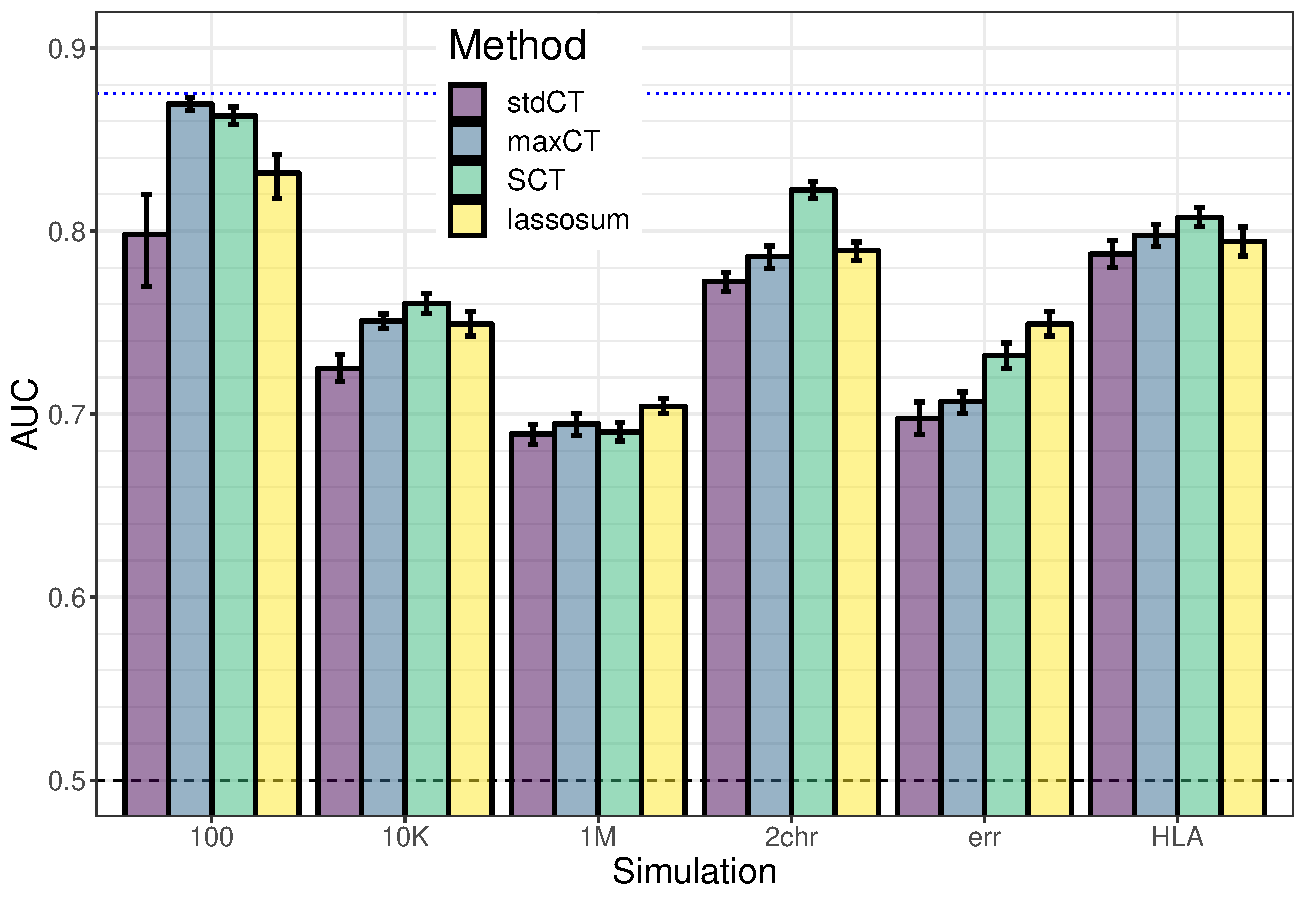
\includegraphics[width=0.8\textwidth]{AUC-simus.pdf}}
\caption{Results of the 6 simulation scenarios: (100) 100 random causal SNPs; (10K) 10,000 random causal SNPs; (1M) all 1M SNPs are causal SNPs; (2chr) 100 SNPs of chromosome 1 are causal and all SNPs of chromosome 2, with half of the heritability for both chromosomes; (err) 10,000 random causal SNPs, but 10\% of the GWAS effects are reported with an opposite effect; (HLA) 7105 causal SNPs in some long-range LD region of chromosome 6. Mean and 95\% CI of $10^4$ non-parametric bootstrap replicates of the mean AUC of 10 simulations for each scenario. The blue dotted line represents the maximum achievable AUC for these simulations (87.5\% for a prevalence of 10\% and an heritability of 50\% -- see equation (3) of \cite{wray2010genetic}).}
\label{fig:AUC-simus}
\end{figure}

\subsection{Real summary statistics}

In figure \ref{fig:AUC-real} and table \ref{tab:AUC}, we report AUC values on the test set (mean and 95\% CI from $10^4$ bootstrap samples) and the number of variants used in the final model.



[TALK ABOUT PARAMETERS FOR 10 BEST PREDICTIONS??]

Effects resulting from SCT have mostly the same sign as initial effects from GWAS, with some effects being largely unchanged, and others having an effect that is shrunk to 0 or completely 0, i.e.\ variants not included in the final model (Figures \ref{fig:neweffreal} and \ref{fig:neweffsimu}).
[TALK ABOUT PARTICULAR CASES]
[METTRE RESULTS FIG S2 AVANT?]


\begin{figure}[h]
\centerline{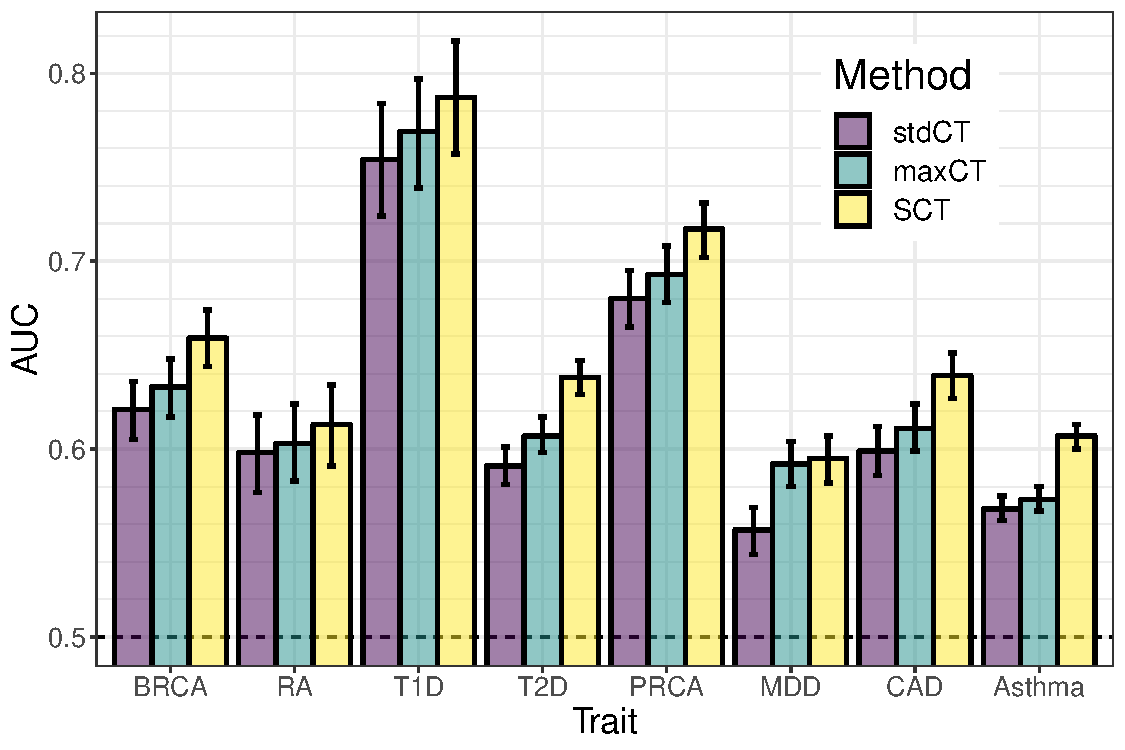
\includegraphics[width=0.8\textwidth]{AUC-real.pdf}}
\caption{AUC values on the test set of UKBB (mean [95\% CI] from $10^4$ bootstrap samples). See corresponding values in table \ref{tab:AUC}.}
\label{fig:AUC-real}
\end{figure}

%%%%%%%%%%%%%%%%%%%%%%%%%%%%%%%%%%%%%%%%%%%%%%%%%%%%%%%%%%%%%%%%%%%%%%%%%%%%%%%%

\section{Discussion}

[TODO results]

\subsection{Limitations of the study}

We analyze 8 different binary phenotypes in this study; there are more to be analyzed. For example, for psychiatric disease, we include only depression (MDD) because diseases such as schyzophrenia and bipolar disorder have very few cases in the UK Biobank; dedicated datasets should be used to assess effectiveness of maxCT and SCT for such diseases. 
We also do not analyze many automimmune diseases as summary statistics are often outdated in terms of sample size and number of imputed variants\footnote{https://www.immunobase.org/downloads/protected\_data/GWAS\_Data/} and, because there are usually large effects on chromosome 6, methods that use individual-level data are likely to provide better predictive models \cite[]{prive2019efficient}.
We also voluntarily do not analyze any continuous trait such as height or BMI because there are many individual-level data available for such phenotypes and methods directly using individual-level data are likely to provide better predictive models than the ones using summary statistics \cite[]{prive2019efficient}. 
Phenotypes with minuscule effects such as educational attainment for which huge GWAS summary statistics are available might be an exception \cite[]{lee2018gene}.

Moreover, we focus this study on improving the C+T method. The C+T method is by far the simplest and most widely-used method for constructing polygenic risk scores based on summary statistics. The idea behind C+T is really simple because it directly uses weights learned from GWAS; it further removes SNPs as one does when reporting hits from GWAS, i.e.\ only SNPs that pass the genome-wide threshold (p-value thresholding) and that are independent association findings (clumping) are reported. 
Yet, there are two other established methods based on summary statistics: LDpred and lassosum, but do not provide much better predictions as compared to stdCT \cite[]{vilhjalmsson2015modeling,mak2017polygenic,allegrini2019genomic}. Other methods are emerging such as ...; they are not very easy to use, nor easy to understand, nor they perform much better than stdCT. [CITE OTHERS?? BE NICE??]

\subsection{Areas of improvement}

There are many ways to improve prediction further. For example, developing techniques that can handle errors should be of great interest \cite[]{smith2011improving,bolin2014supervised}. There are many applications in medical data: mistakes in meta-analyses results \cite[]{greco2013meta}, mistakes in identifying diseases \cite[]{wray2012impact,thomas2018frequency}, defining ambiguous alleles \cite[]{chen2018prs}.
For example, in one simulation scenario (``err'') of this paper, we show that having an extra layer of training consisting in stacking C+T models makes it possible to partially correct for mistakes. 
%We have also remarked improved prediction for SCT when including ambiguous alleles for real phenotypes while maxCT would decrease (data not shown). [CITE CORRESPONDING PHENOTYPES]

As for the SCT method itself, the stacking step can be used for either binary or continuous phenotypes. 
Yet, it makes sense to use age in the models, using for example Cox proportional-hazards model to predict age of disease onset, with possibly censored data \cite[]{cox1972regression}.
Cox regression has already proven useful for increasing power in GWAS \cite[]{hughey2019cox}.
Cox model is not implemented yet as part as our efficient penalized regression implementation, only linear and logistic regressions are. This is an area of future development; at the moment, if sample size is not too large, one could use R package glmnet to implement stacking based on Cox model \cite[]{tibshirani2012strong}.

One might also want to use other information such as sex or ancestry (using principal components). Indeed, it is easy to add those in the stacking step as (unpenalized) variables in the penalized logistic regression. Yet, we have to be cautious doing so. For example, because prevalence of CAD is much higher in men than in women in the UKBB (8-9\% vs 2\%), adding sex in the model amount to fitting two different intercepts, centering distributions of fitted probabilities around disease prevalence (Figure \ref{fig:sexCAD}). This increases the AUC from 63.9\% to 74.4\% but results in a model that would classify all women as healthy. A possible solution would be to report AUC figures for each gender separately, or even to fit a model for each gender separately (in the stacking step).
Fitting models separately would enable the use of sex chromosomes without introducing bias. 
As for ancestry concerns, fitting different models for different ancestries might be a way to get more calibrated results and to account for differences in effect sizes and LD. 
However, here for CAD, fitting two separate models results in a slight loss of predictive performance, while using variable `sex' does not change results when they are reported for each gender separately, with an AUC of 64.9\% [63.5-66.3] for men and 62.5\% [59.8-65.2] for women.
Thus, adding `sex' as a covariate in the model may provide a model with similar discrimination and with better calibration of probabilities (if prevalence in the data is representative of prevalence in the population). Yet, we would like to emphasize again that reporting one AUC figure for all individuals would be misleading in the case of using variable `sex' in the model.


\subsection{Conclusion}

[TODO]

%%%%%%%%%%%%%%%%%%%%%%%%%%%%%%%%%%%%%%%%%%%%%%%%%%%%%%%%%%%%%%%%%%%%%%%%%%%%%%%%

\newpage

\section*{Acknowledgements}

Authors acknowledge LabEx PERSYVAL-Lab (ANR-11-LABX-0025-01) and ANR project FROGH (ANR-16-CE12-0033). Authors also acknowledge the Grenoble Alpes Data Institute that is supported by the French National Research Agency under the ``Investissements d'avenir'' program (ANR-15-IDEX-02).
This research has been conducted using the UK Biobank Resource under Application Number 25589.

%%%%%%%%%%%%%%%%%%%%%%%%%%%%%%%%%%%%%%%%%%%%%%%%%%%%%%%%%%%%%%%%%%%%%%%%%%%%%%%%

\newpage

\bibliographystyle{natbib}
\bibliography{refs}

%%%%%%%%%%%%%%%%%%%%%%%%%%%%%%%%%%%%%%%%%%%%%%%%%%%%%%%%%%%%%%%%%%%%%%%%%%%%%%%%

\newpage
\section*{Supplementary Data}

\renewcommand{\thefigure}{S\arabic{figure}}
\setcounter{figure}{0}
\renewcommand{\thetable}{S\arabic{table}}
\setcounter{table}{0}

\begin{figure}[htb]
\centerline{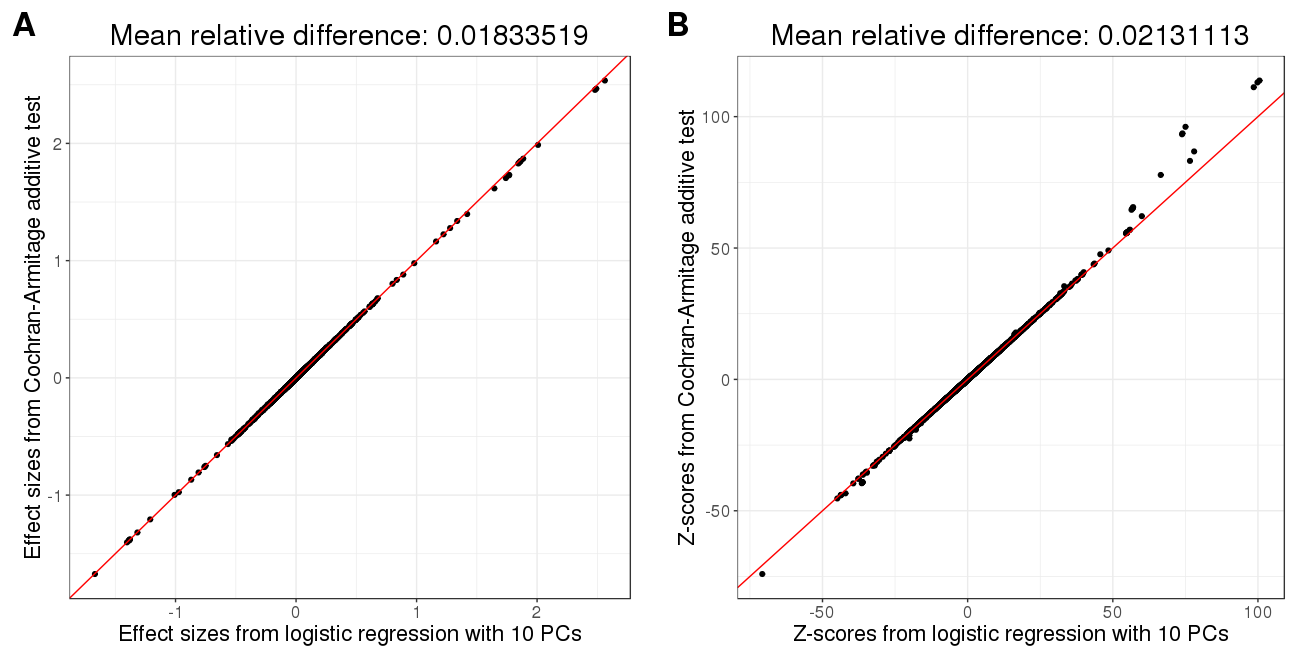
\includegraphics[width=0.95\textwidth]{equivalence.png}}
\caption{Comparison of estimated effect sizes (\textbf{A}) and Z-scores (\textbf{B}) if computed using a logistic regression with 10 principal components as covariates, or with a simple Cochran-Armitage additive test. Phenotypes were simulated using 100 causal SNPs only, allowing for large effects.}
\label{fig:GWAS}
\end{figure}

%%%%%%%%%%%%%%%%%%%%%%%%%%%%%%%%%%%%%%%%%%%%%%%%%%%%%%%%%%%%%%%%%%%%%%%%%%%%%%%%

\begin{table}[h]
\caption{AUC values on the test set of UKBB (mean [95\% CI] from $10^4$ bootstrap samples) and the number of variants used in the final model.\label{tab:AUC}}
\vspace*{0.5em}
\centering
\begin{tabular}{|l|c|c|c|c|}
  \hline
Trait & stdCT & maxCT & SCT \\
  \hline
Breast cancer (BRCA) & 62.1 [60.5-63.6] & 63.3 [61.7-64.8] & 65.9 [64.4-67.4] \\
 & 6256 & 2572 & 670,050 \\
Rheumatoid arthritis (RA) & 59.8 [57.7-61.8] & 60.3 [58.3-62.4] & 61.3 [59.1-63.4] \\
 & 12,220 & 88,556 & 317,456 \\
Type 1 diabetes (T1D) & 75.4 [72.4-78.4] & 76.9 [73.9-79.7] & 78.7 [75.7-81.7] \\
 & 1112 & 267 & 135,991 \\
Type 2 diabetes (T2D) & 59.5 [58.5-60.5] & 60.7 [59.8-61.6] & 63.8 [62.9-64.8] \\
 & 252 & 33,238 & 535,785 \\
Prostate cancer (PRCA) & & & \\
 & & & \\
Depression (MDD) & 53.9 [52.6-55.2] & 59.6 [58.3-60.8] & 59.8 [58.5-61.0] \\
 & 170,505 & 205,096 & 473,333 \\
Coronary artery disease (CAD) & 59.9 [58.6-61.2] & 61.1 [59.9-62.4] & 63.9 [62.7-65.1] \\
 & 1182 & 87,577 & 315,165 \\
Asthma & & & \\
 & & & \\
   \hline
\end{tabular}
\end{table}

%%%%%%%%%%%%%%%%%%%%%%%%%%%%%%%%%%%%%%%%%%%%%%%%%%%%%%%%%%%%%%%%%%%%%%%%%%%%%%%%

\begin{figure}[htb]
\centering
\begin{subfigure}[b]{0.7\textwidth}
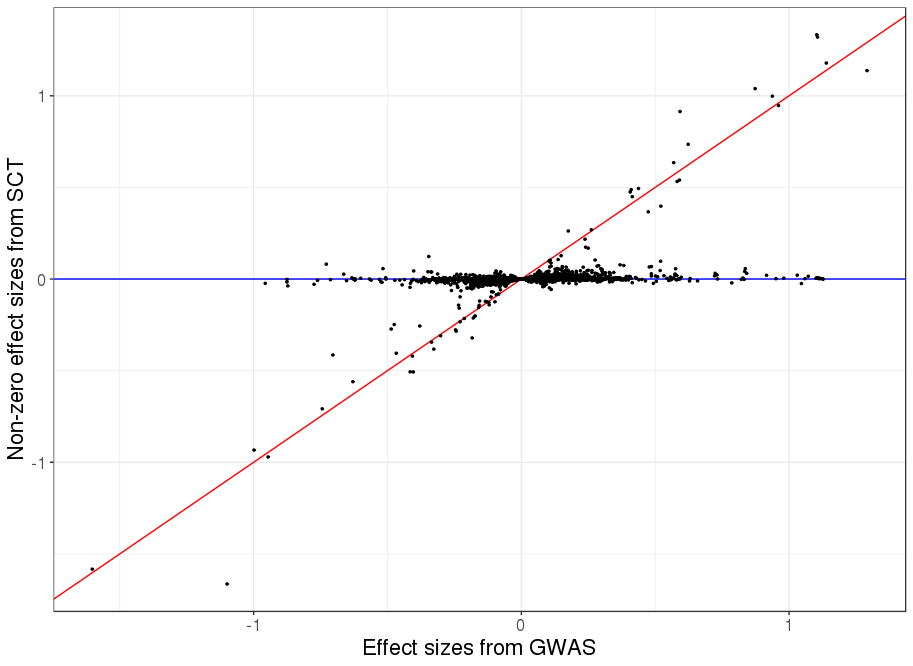
\includegraphics[width=\textwidth]{new-effects-simu100.png}
\caption{100 random causal SNPs}
\end{subfigure}
\\~\\~\\
\begin{subfigure}[b]{0.7\textwidth}
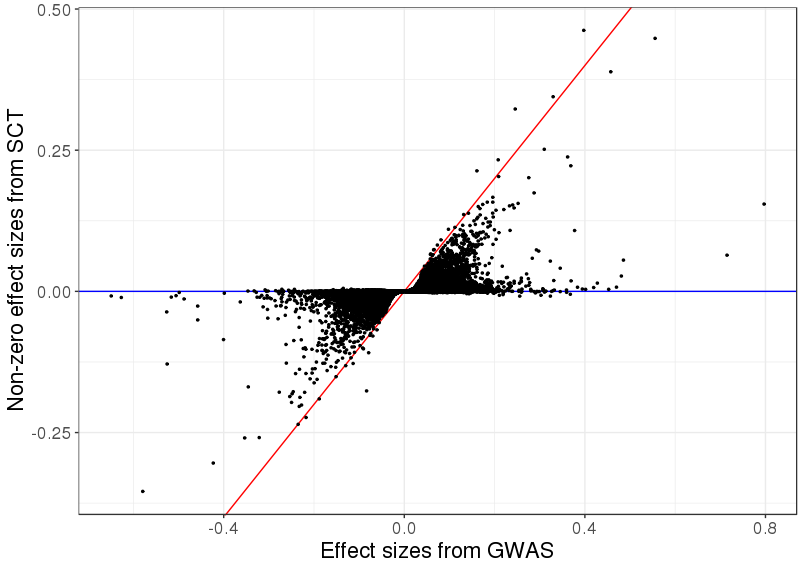
\includegraphics[width=\textwidth]{new-effects-simu10K.png}
\caption{10,000 random causal SNPs}
\end{subfigure}
\end{figure}

\begin{figure}[htb]\ContinuedFloat
\centering
\begin{subfigure}[b]{0.7\textwidth}
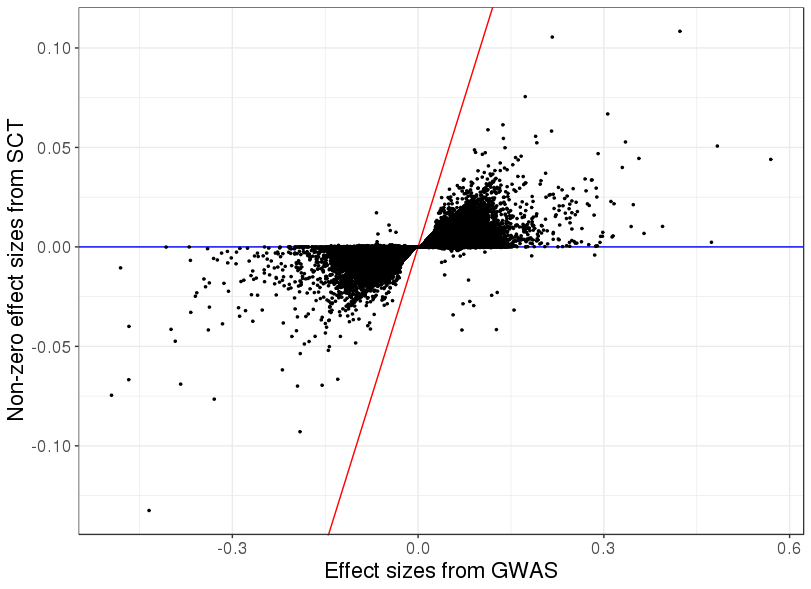
\includegraphics[width=\textwidth]{new-effects-simu1M.png}
\caption{all 1M SNPs are causal SNPs}
\end{subfigure}
\\~\\~\\
\begin{subfigure}[b]{0.7\textwidth}
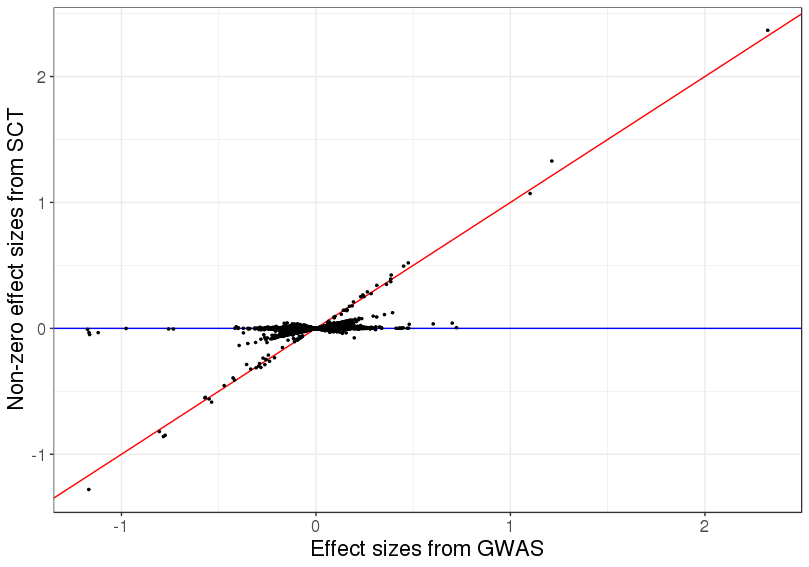
\includegraphics[width=\textwidth]{new-effects-simu2chr.png}
\caption{Causal SNPs on chromosomes 1 \& 2}
\end{subfigure}
\end{figure}

\begin{figure}[htb]\ContinuedFloat
\centering
\begin{subfigure}[b]{0.7\textwidth}
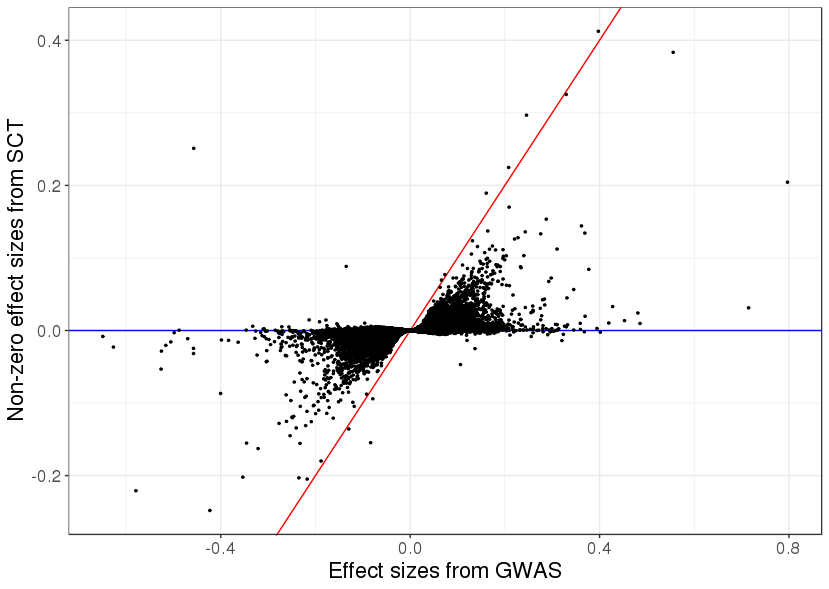
\includegraphics[width=\textwidth]{new-effects-simuerr.png}
\caption{10,000 random causal SNPs, but 10\% of the GWAS effects are reported with an opposite effect}
\end{subfigure}
\\~\\~\\
\begin{subfigure}[b]{0.7\textwidth}
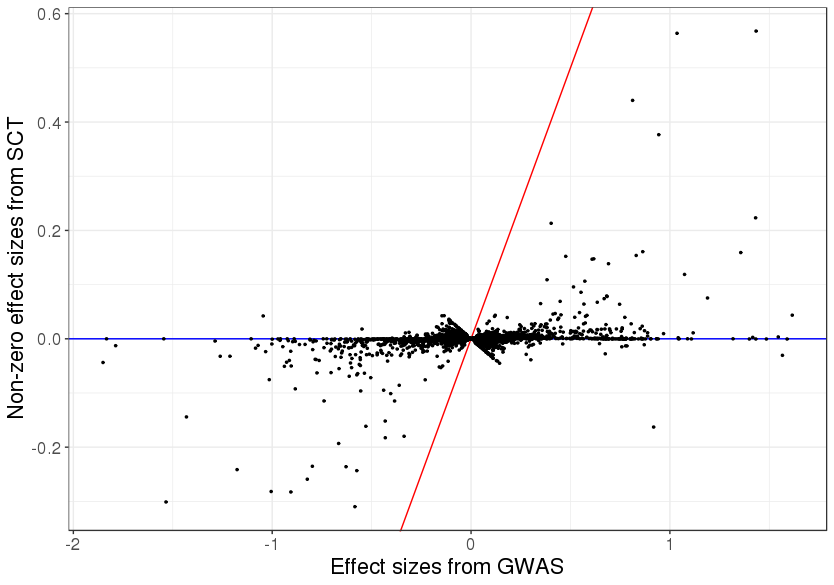
\includegraphics[width=\textwidth]{new-effects-simuHLA.png}
\caption{7105 causal SNPs in some long-range LD region of chromosome 6.}
\end{subfigure}

\caption{New effect sizes resulting from SCT versus initial effect sizes of GWAS in the first simulation of each simulation scenario. Only non-zero effects are represented. Red line corresponds to the 1:1 line.}
\label{fig:neweffsimu}
\end{figure}

%%%%%%%%%%%%%%%%%%%%%%%%%%%%%%%%%%%%%%%%%%%%%%%%%%%%%%%%%%%%%%%%%%%%%%%%%%%%%%%%

\begin{figure}[htb]
\centering
\begin{subfigure}[b]{\textwidth}
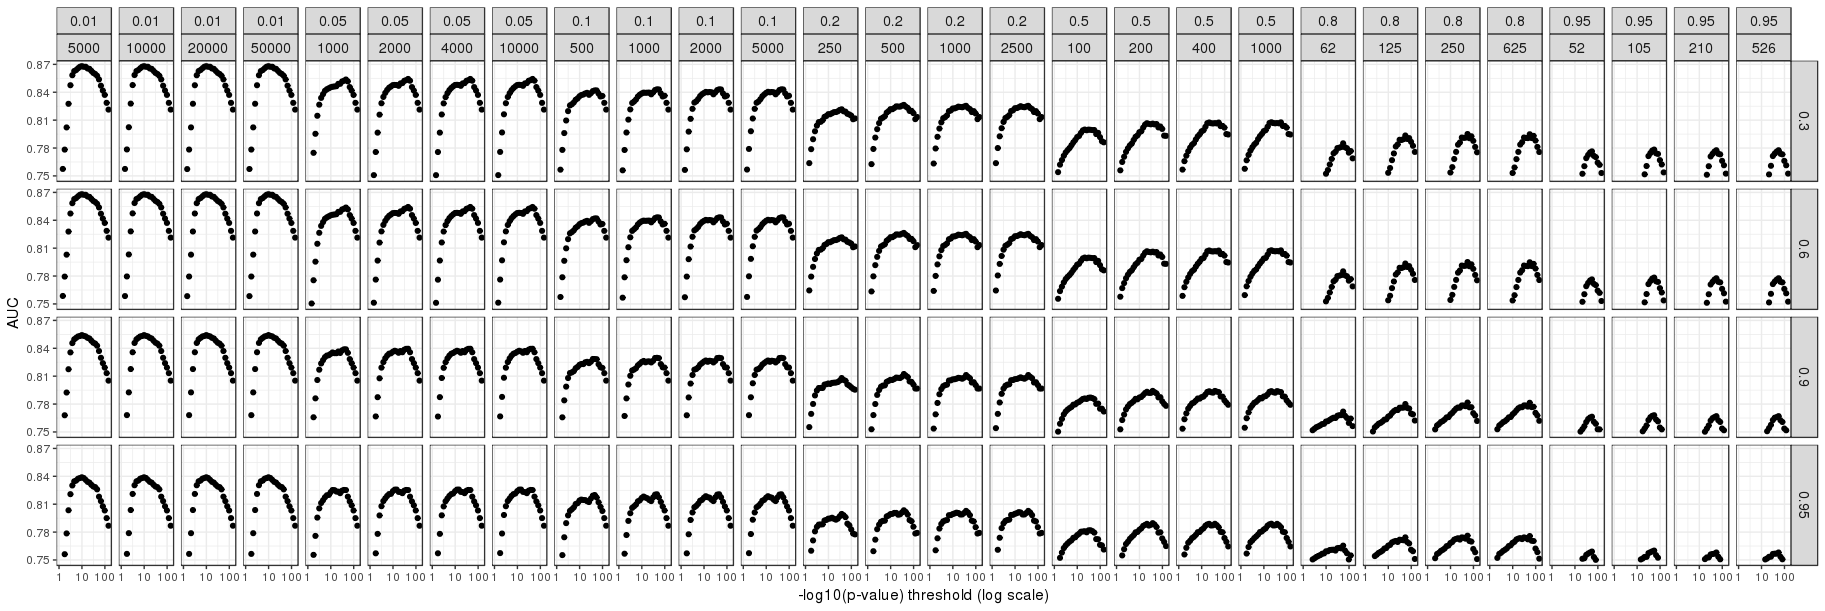
\includegraphics[width=\textwidth]{grid-simu100.png}
\caption{100 random causal SNPs\label{fig:simugridA}}
\end{subfigure}
\\~\\~\\
\begin{subfigure}[b]{\textwidth}
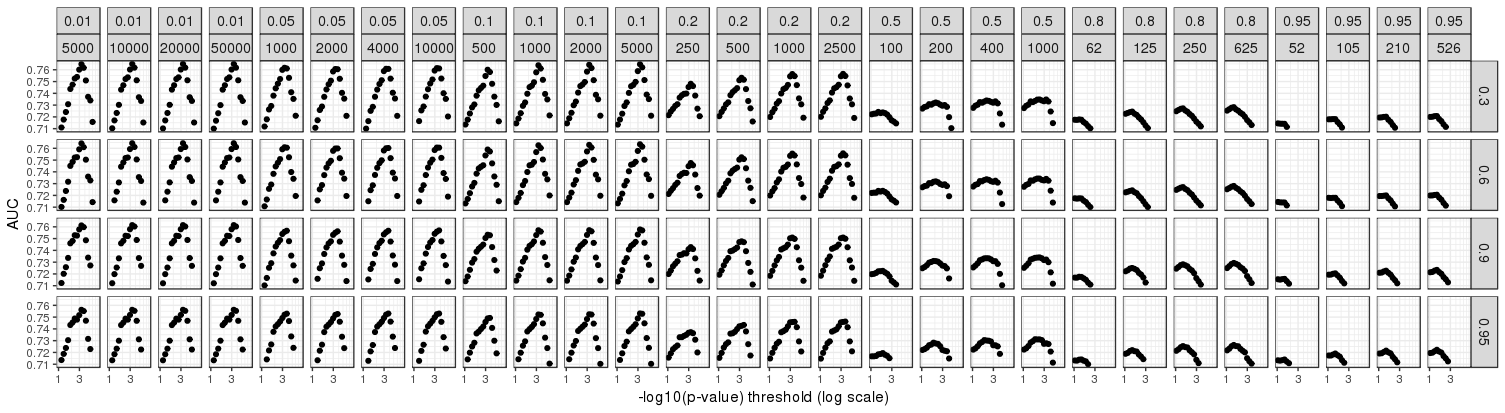
\includegraphics[width=\textwidth]{grid-simu10K.png}
\caption{10,000 random causal SNPs\label{fig:simugridB}}
\end{subfigure}
\\~\\~\\
\begin{subfigure}[b]{\textwidth}
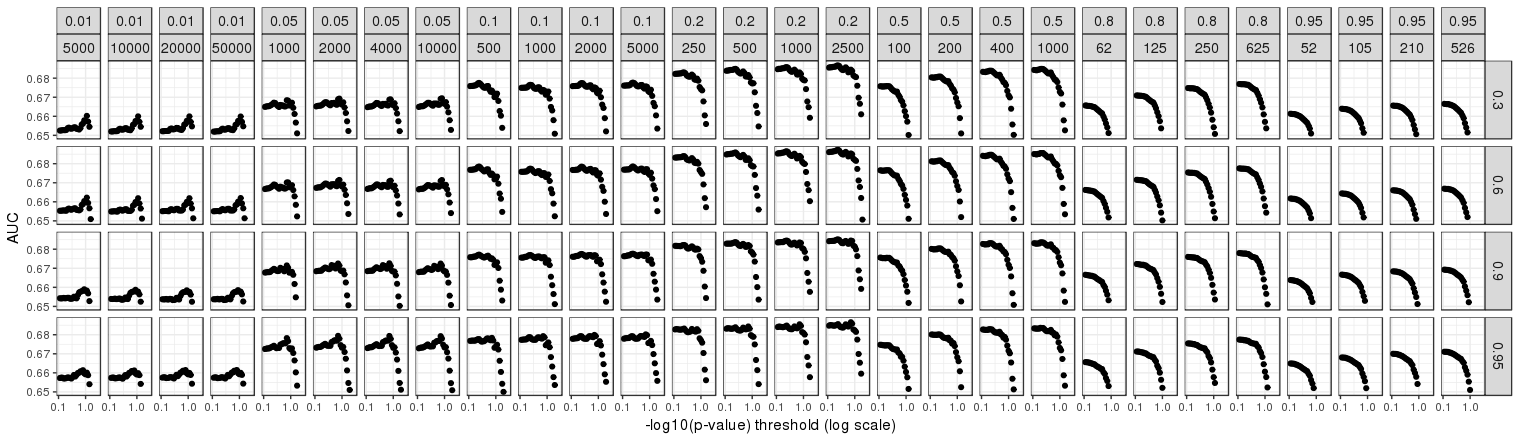
\includegraphics[width=\textwidth]{grid-simu1M.png}
\caption{all 1M SNPs are causal SNPs\label{fig:simugridC}}
\end{subfigure}
\end{figure}

\begin{figure}[htb]\ContinuedFloat
\centering
\begin{subfigure}[b]{\textwidth}
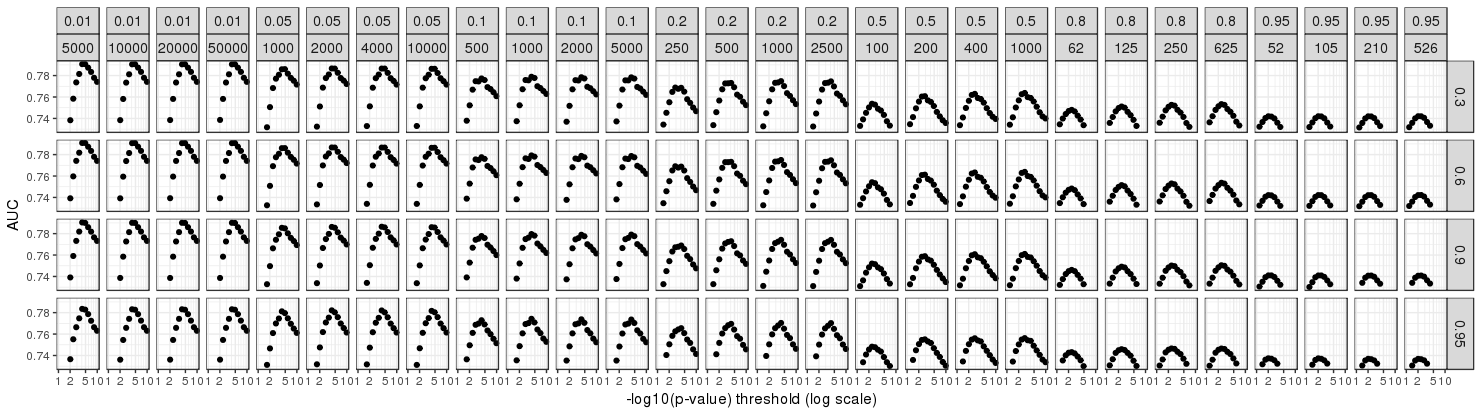
\includegraphics[width=\textwidth]{grid-simu2chr.png}
\caption{Causal SNPs on chromosomes 1 \& 2}
\end{subfigure}
\\~\\~\\
\begin{subfigure}[b]{\textwidth}
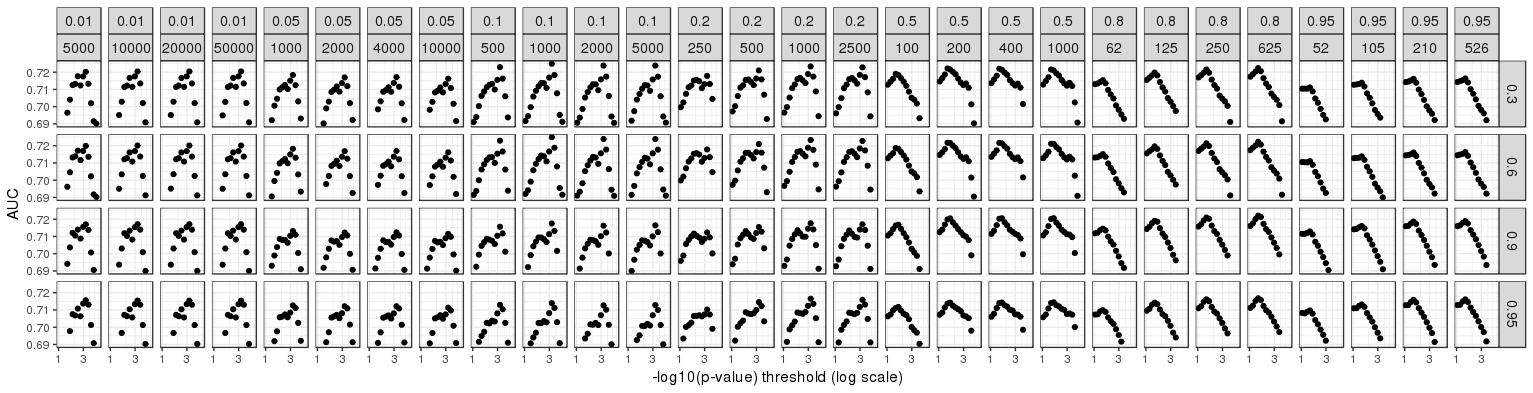
\includegraphics[width=\textwidth]{grid-simuerr.png}
\caption{10,000 random causal SNPs, but 10\% of the GWAS effects are reported with an opposite effect}
\end{subfigure}
\\~\\~\\
\begin{subfigure}[b]{\textwidth}
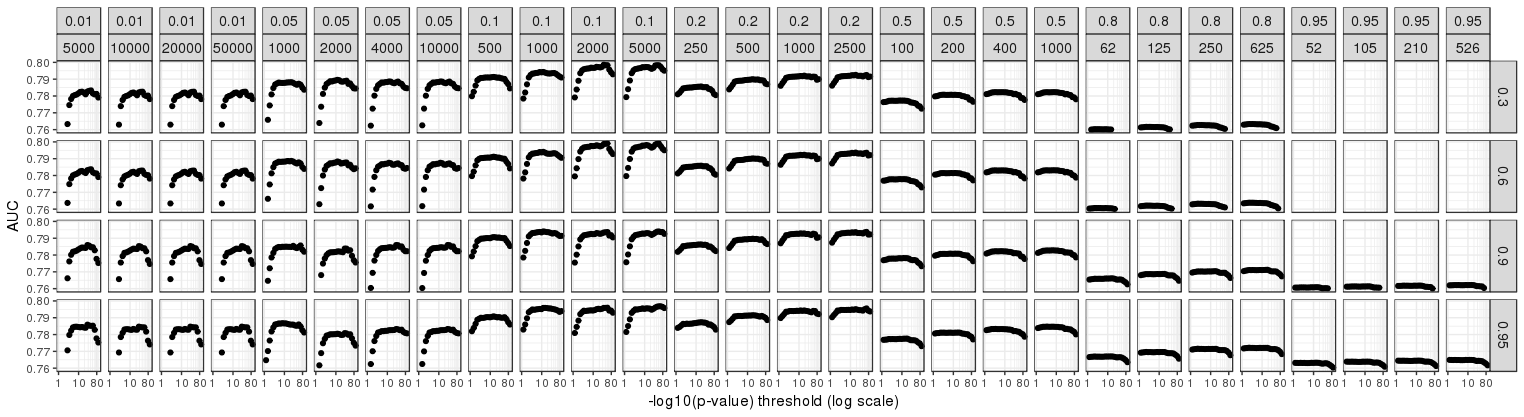
\includegraphics[width=\textwidth]{grid-simuHLA.png}
\caption{7105 causal SNPs in some long-range LD region of chromosome 6.}
\end{subfigure}

\caption{AUC values (for the training set) when predicting disease status for many parameters of C+T in the first simulation of each simulation scenario. Facets are presenting different clumping thresholds $r_{c}^2$ from 0.01 to 0.95, window sizes $w_c$ from 52 to 50,000 kb, and imputation thresholds from 0.3 to 0.95. The x-axis corresponds to the remaining hyper-parameter, the p-value threshold $p_T$; here, -log10(p-values) are represented using a logarithmic scale.}
\end{figure}

%%%%%%%%%%%%%%%%%%%%%%%%%%%%%%%%%%%%%%%%%%%%%%%%%%%%%%%%%%%%%%%%%%%%%%%%%%%%%%%%

\begin{figure}[htb]
\centering
\begin{subfigure}[b]{0.7\textwidth}
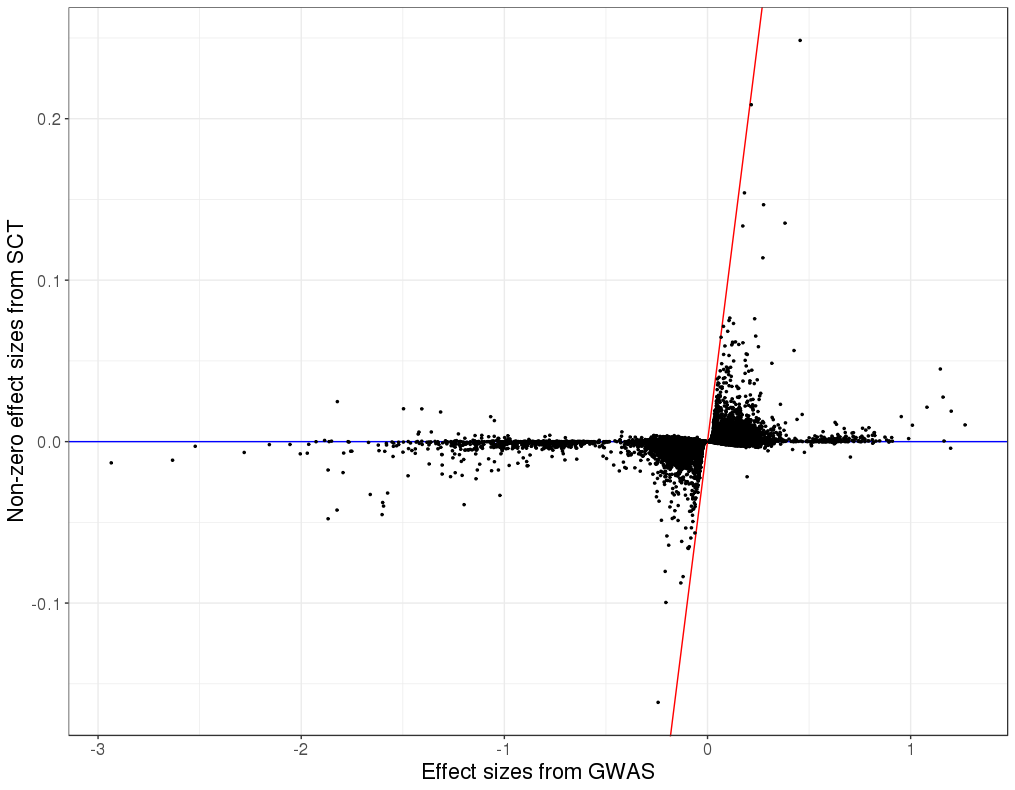
\includegraphics[width=\textwidth]{new-effects-BRCA.png}
\caption{Breast cancer}
\end{subfigure}
\\~\\~\\
\begin{subfigure}[b]{0.7\textwidth}
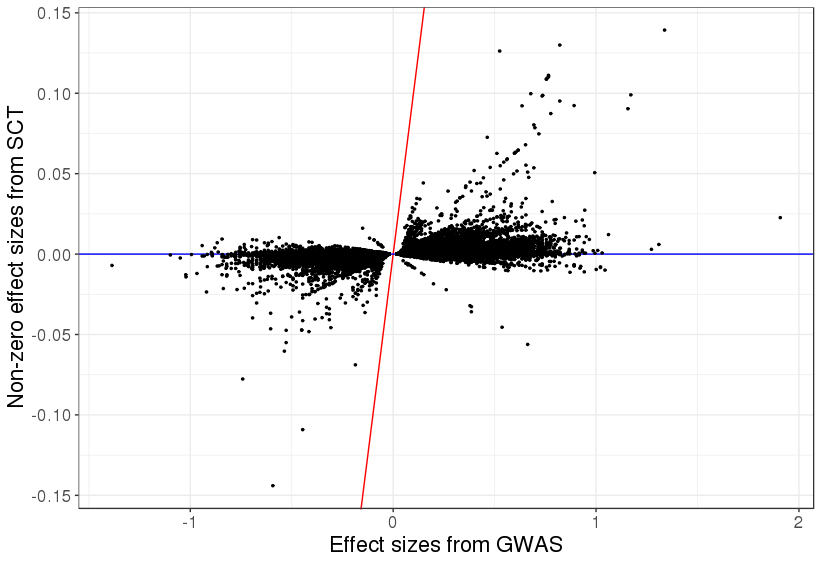
\includegraphics[width=\textwidth]{new-effects-RA.png}
\caption{Rheumatoid arthritis}
\end{subfigure}
\end{figure}

\begin{figure}[htb]\ContinuedFloat
\centering
\begin{subfigure}[b]{0.7\textwidth}
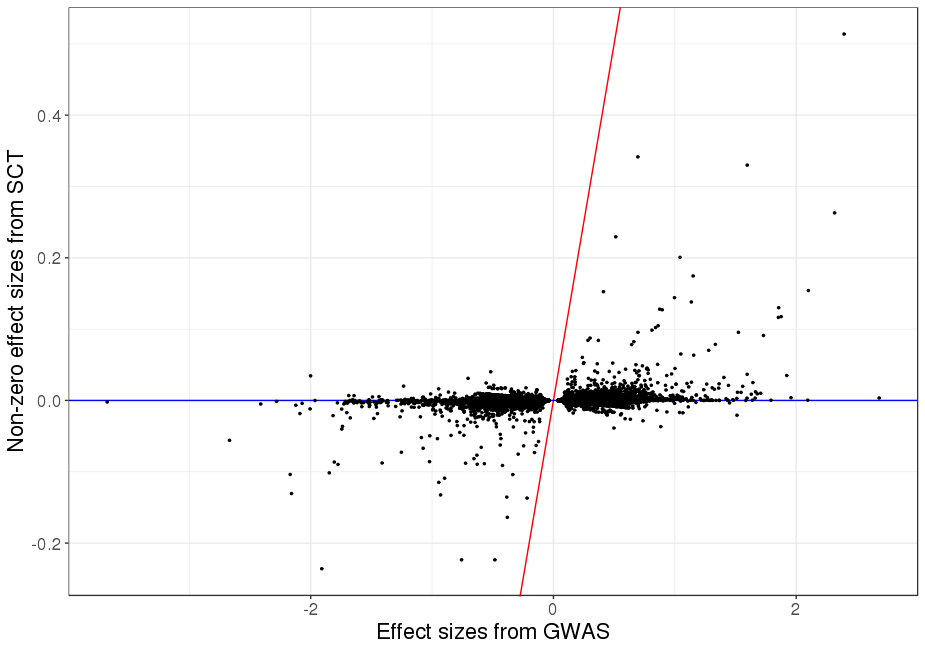
\includegraphics[width=\textwidth]{new-effects-T1D.png}
\caption{Type 1 diabetes}
\end{subfigure}
\\~\\~\\
\begin{subfigure}[b]{0.7\textwidth}
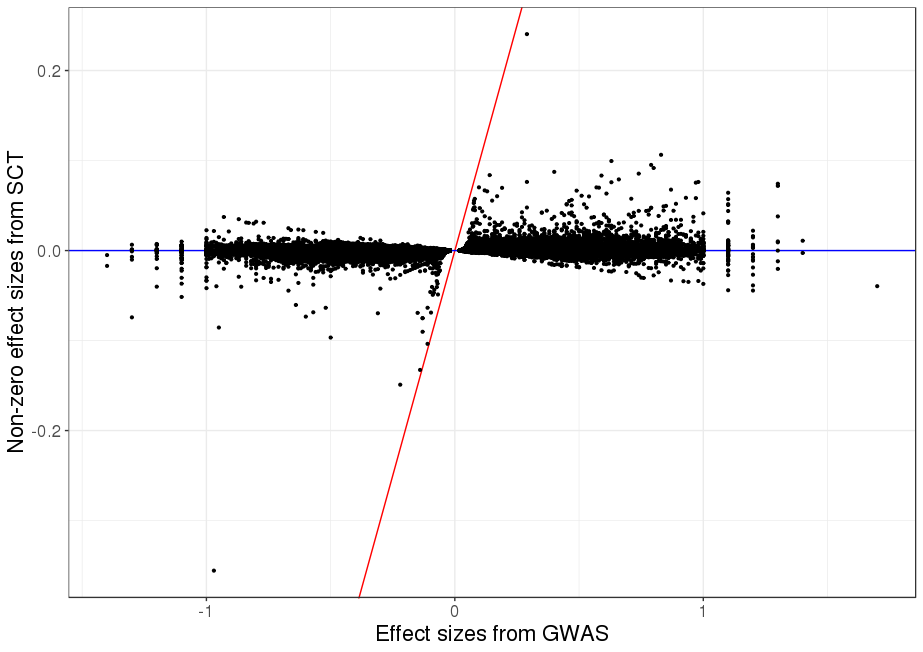
\includegraphics[width=\textwidth]{new-effects-T2D.png}
\caption{Type 2 diabetes}
\end{subfigure}
\end{figure}

\begin{figure}[htb]\ContinuedFloat
\centering
\begin{subfigure}[b]{0.7\textwidth}
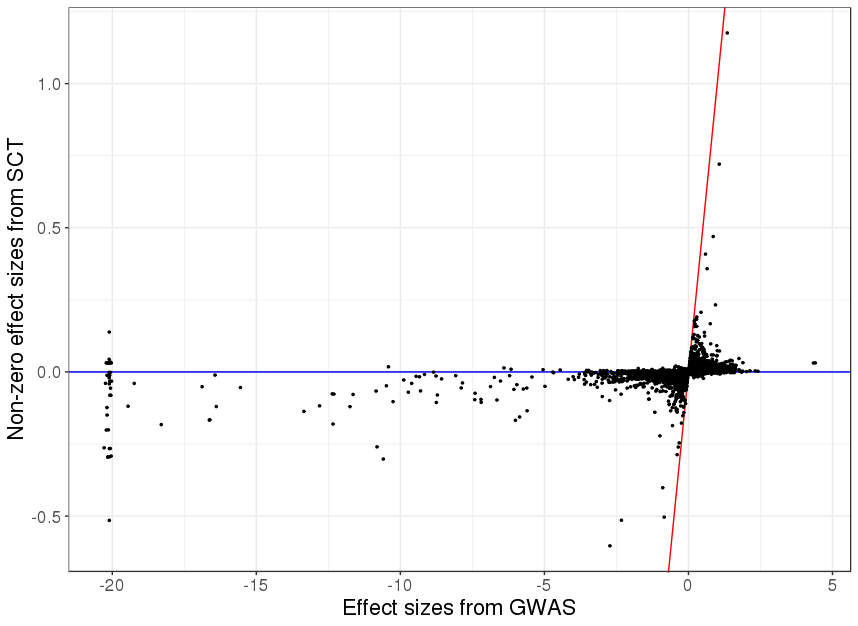
\includegraphics[width=\textwidth]{new-effects-PRCA.png}
\caption{Prostate cancer}
\end{subfigure}
\\~\\~\\
\begin{subfigure}[b]{0.7\textwidth}
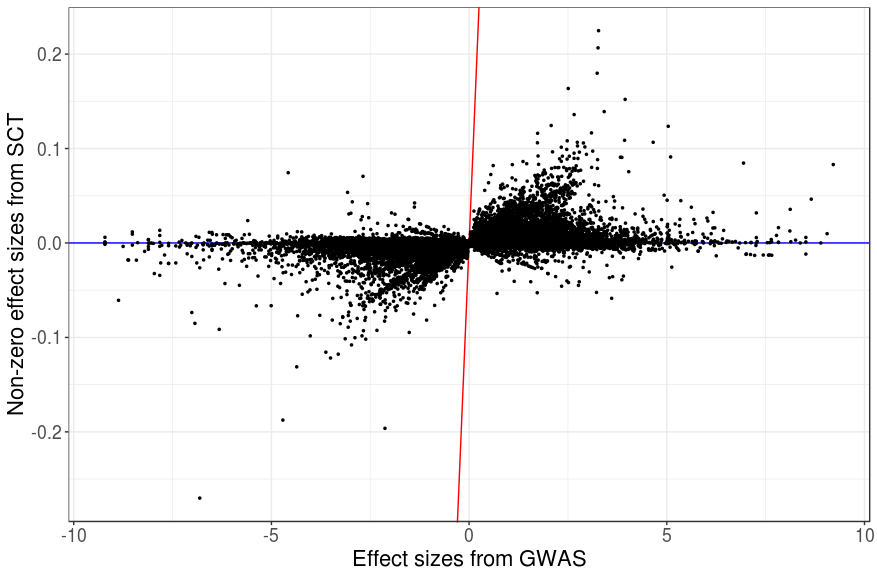
\includegraphics[width=\textwidth]{new-effects-MDD.png}
\caption{Depression}
\end{subfigure}
\end{figure}

\begin{figure}[htb]\ContinuedFloat
\centering
\begin{subfigure}[b]{0.7\textwidth}
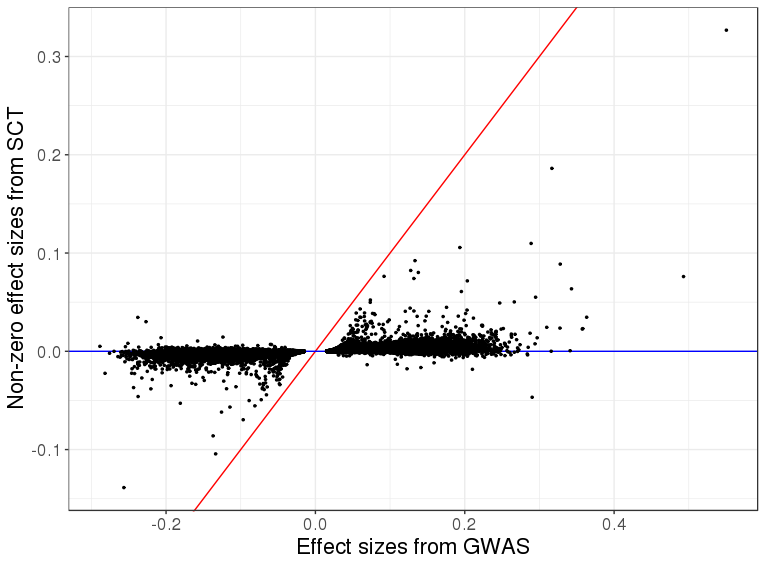
\includegraphics[width=\textwidth]{new-effects-CAD.png}
\caption{Coronary artery disease}
\end{subfigure}
\\~\\~\\
\begin{subfigure}[b]{0.7\textwidth}
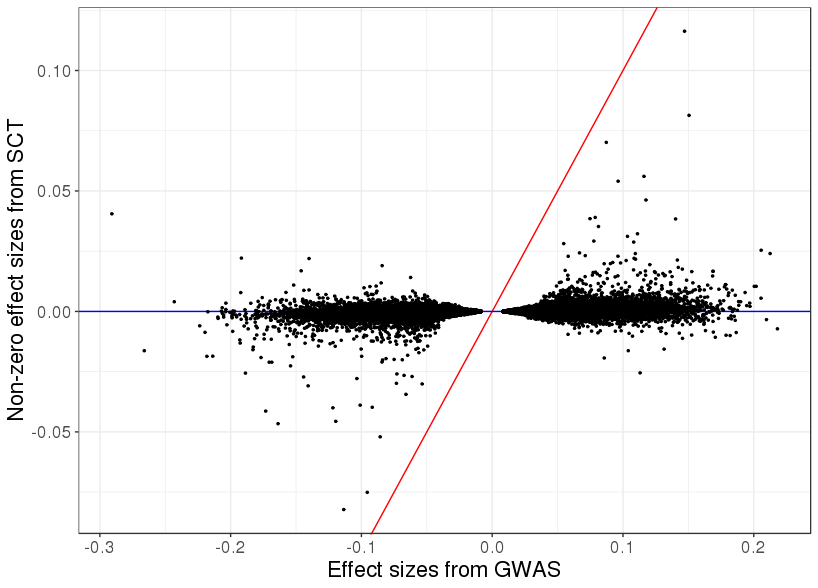
\includegraphics[width=\textwidth]{new-effects-asthma.png}
\caption{Asthma}
\end{subfigure}

\caption{New effect sizes resulting from SCT versus initial effect sizes of GWAS in real data applications. Only non-zero effects are represented. Red line corresponds to the 1:1 line.}
\label{fig:neweffreal}
\end{figure}

%%%%%%%%%%%%%%%%%%%%%%%%%%%%%%%%%%%%%%%%%%%%%%%%%%%%%%%%%%%%%%%%%%%%%%%%%%%%%%%%

\begin{figure}[htb]
\centering
\begin{subfigure}[b]{\textwidth}
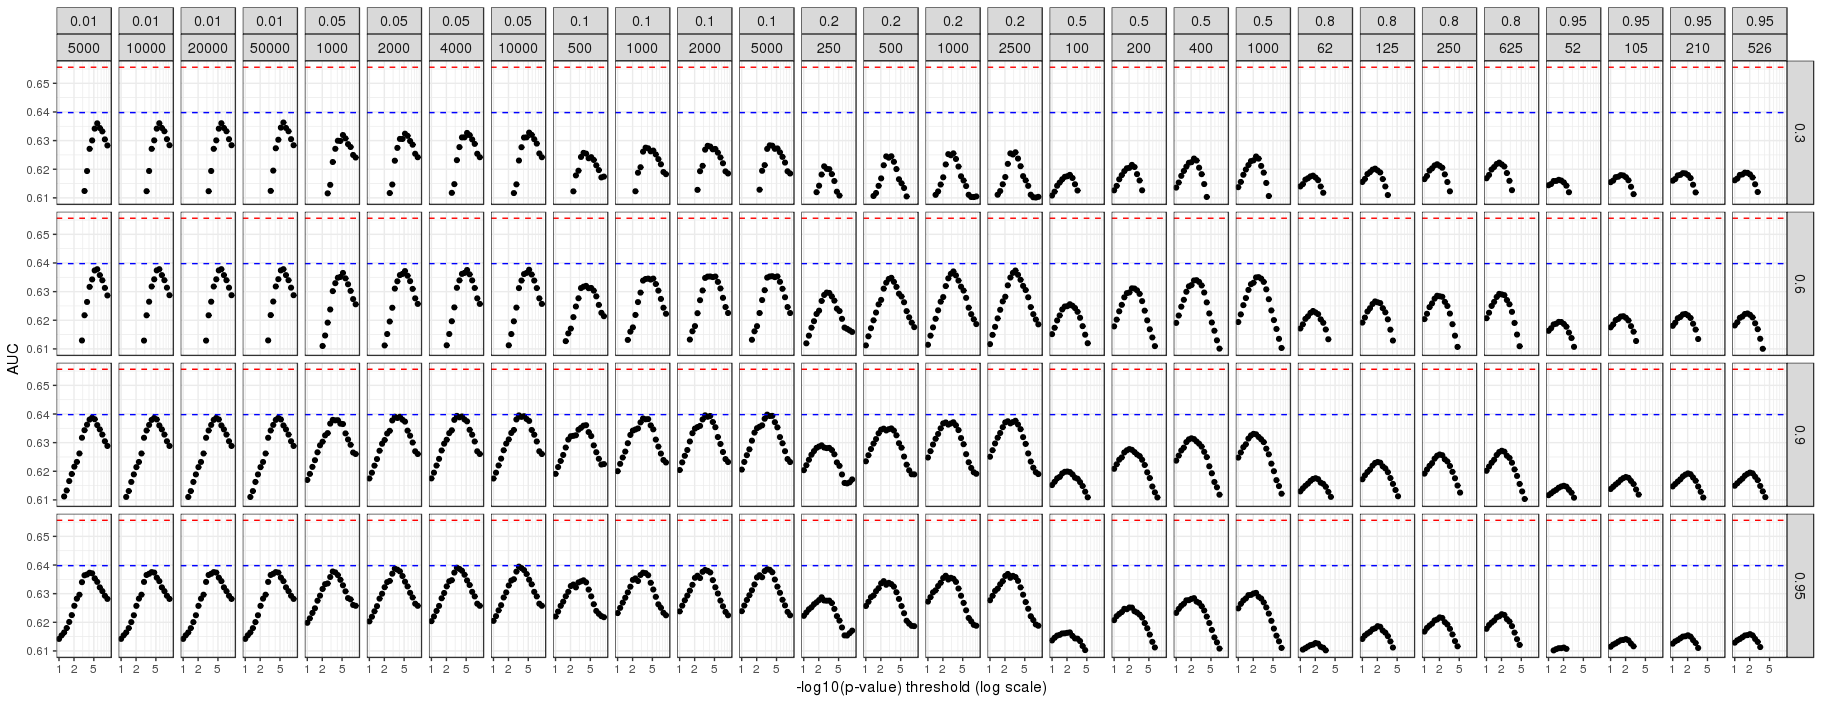
\includegraphics[width=\textwidth]{grid-BRCA.png}
\caption{Breast cancer}
\end{subfigure}
\\~\\
\begin{subfigure}[b]{\textwidth}
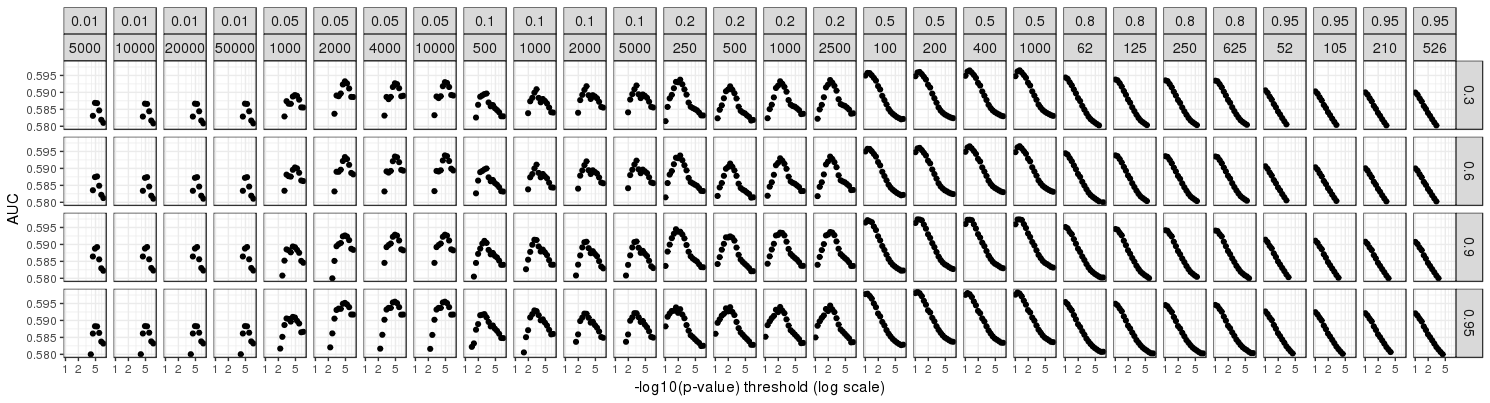
\includegraphics[width=\textwidth]{grid-RA.png}
\caption{Rheumatoid arthritis}
\end{subfigure}
\\~\\
\begin{subfigure}[b]{\textwidth}
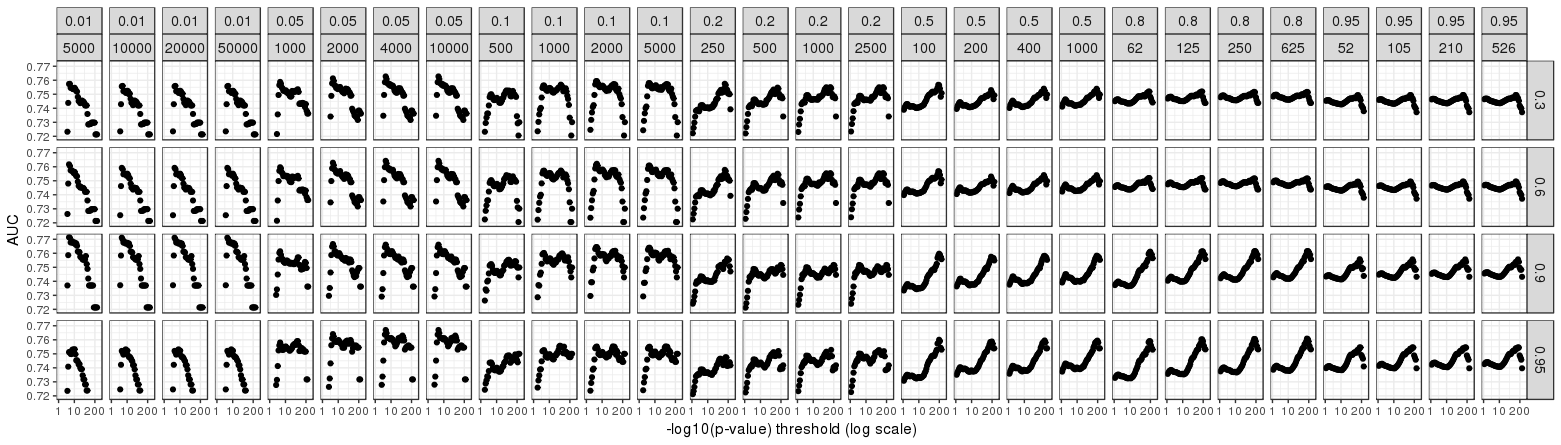
\includegraphics[width=\textwidth]{grid-T1D.png}
\caption{Type 1 diabetes}
\end{subfigure}
\end{figure}

\begin{figure}[htb]\ContinuedFloat
\centering
\begin{subfigure}[b]{\textwidth}
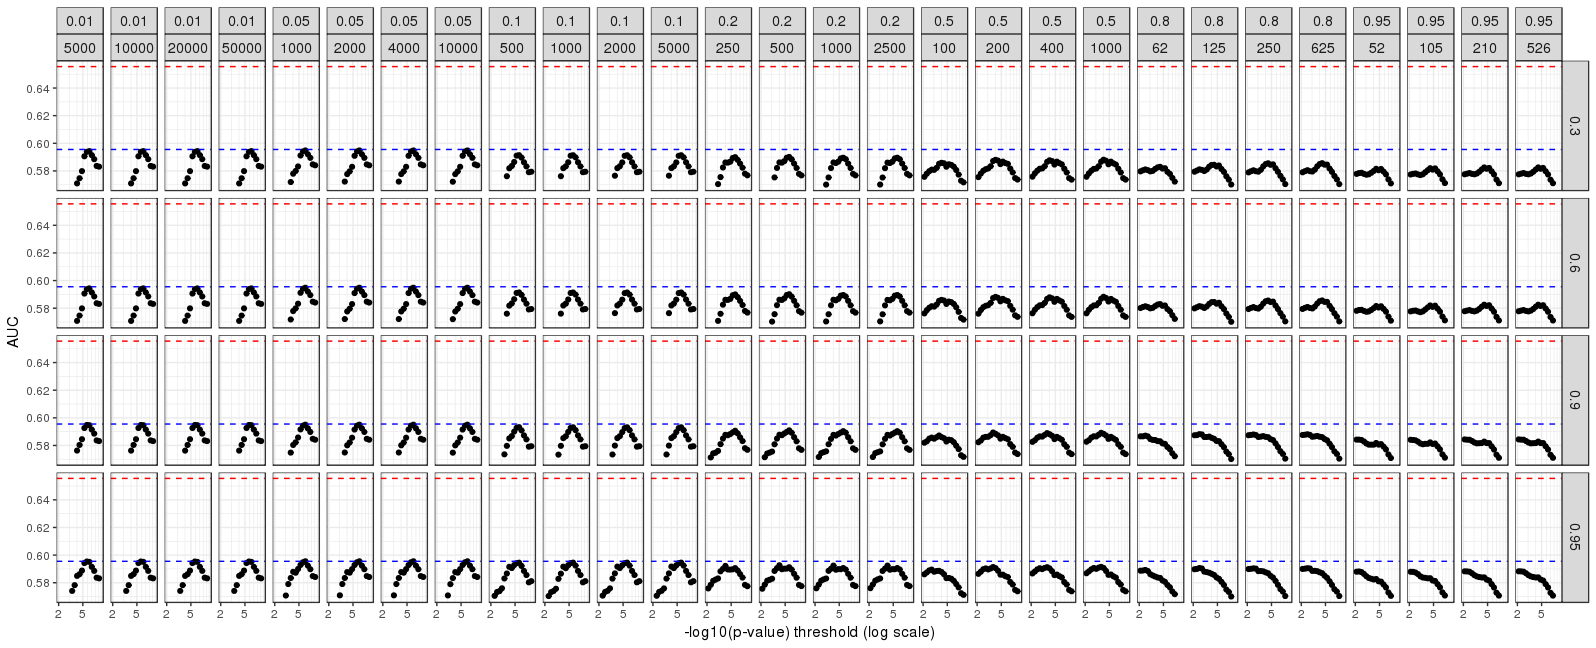
\includegraphics[width=\textwidth]{grid-T2D.png}
\caption{Type 2 diabetes}
\end{subfigure}
\\~\\
\begin{subfigure}[b]{\textwidth}
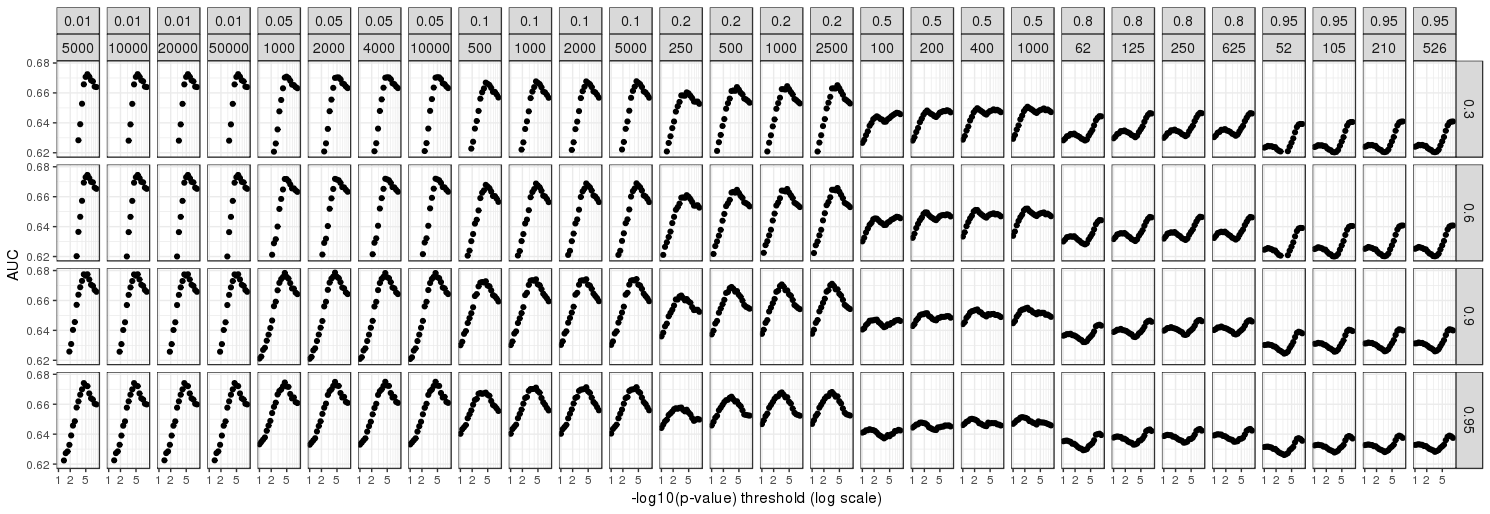
\includegraphics[width=\textwidth]{grid-PRCA.png}
\caption{Prostate cancer}
\end{subfigure}
\\~\\
\begin{subfigure}[b]{\textwidth}
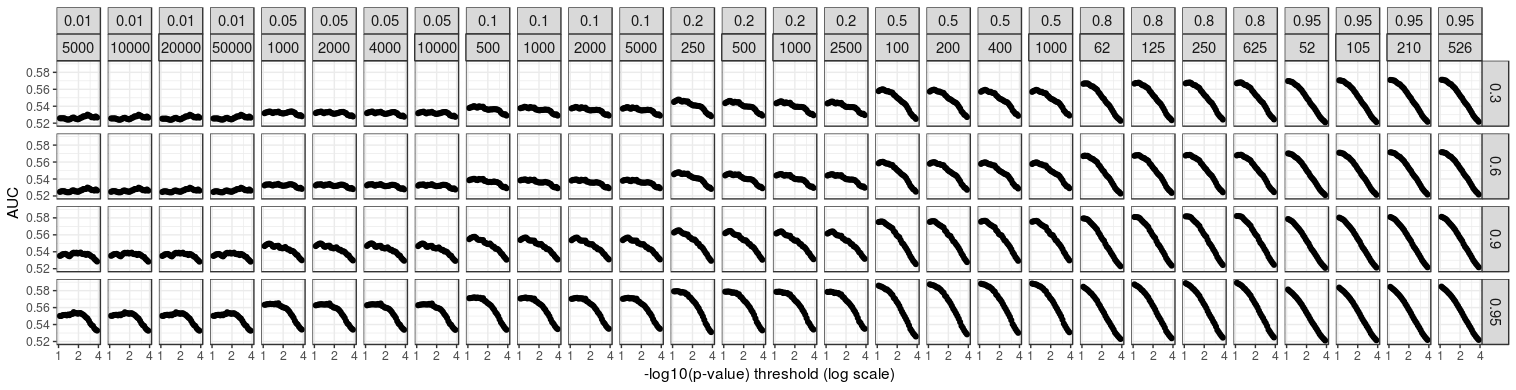
\includegraphics[width=\textwidth]{grid-MDD.png}
\caption{Depression}
\end{subfigure}
\end{figure}

\begin{figure}[htb]\ContinuedFloat
\centering
\begin{subfigure}[b]{\textwidth}
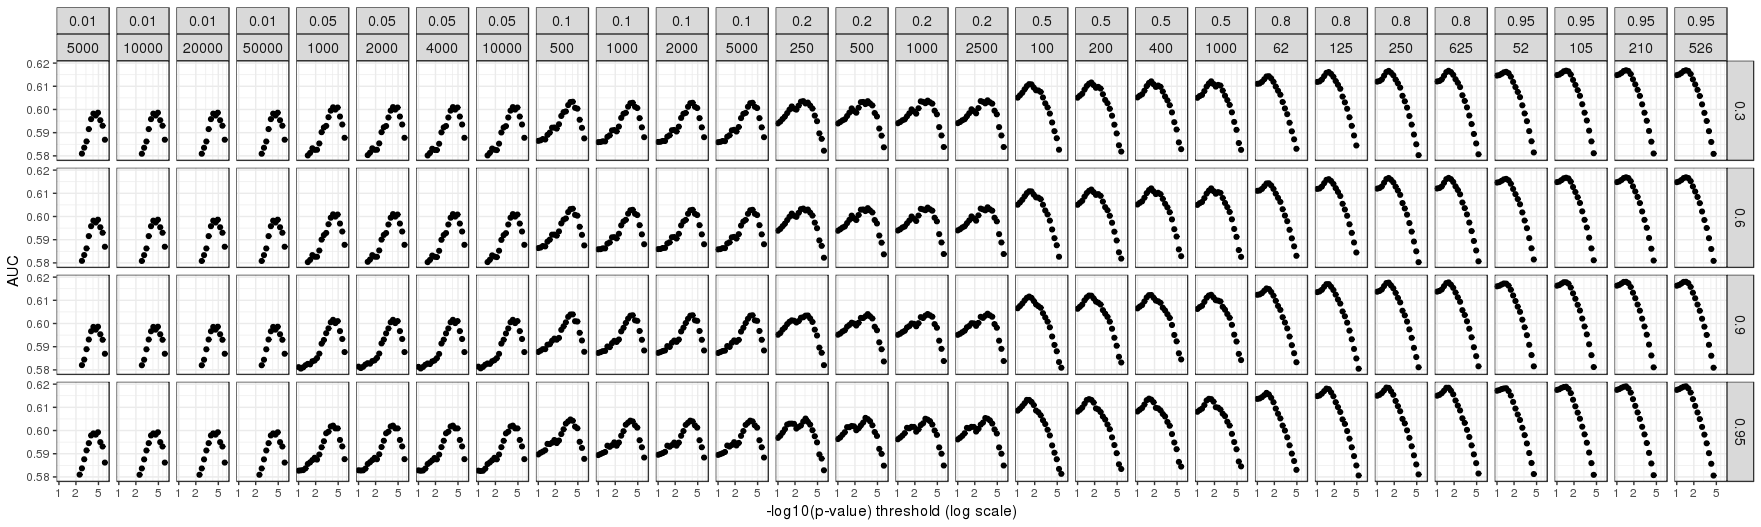
\includegraphics[width=\textwidth]{grid-CAD.png}
\caption{Coronary artery disease}
\end{subfigure}
\\~\\
\begin{subfigure}[b]{\textwidth}
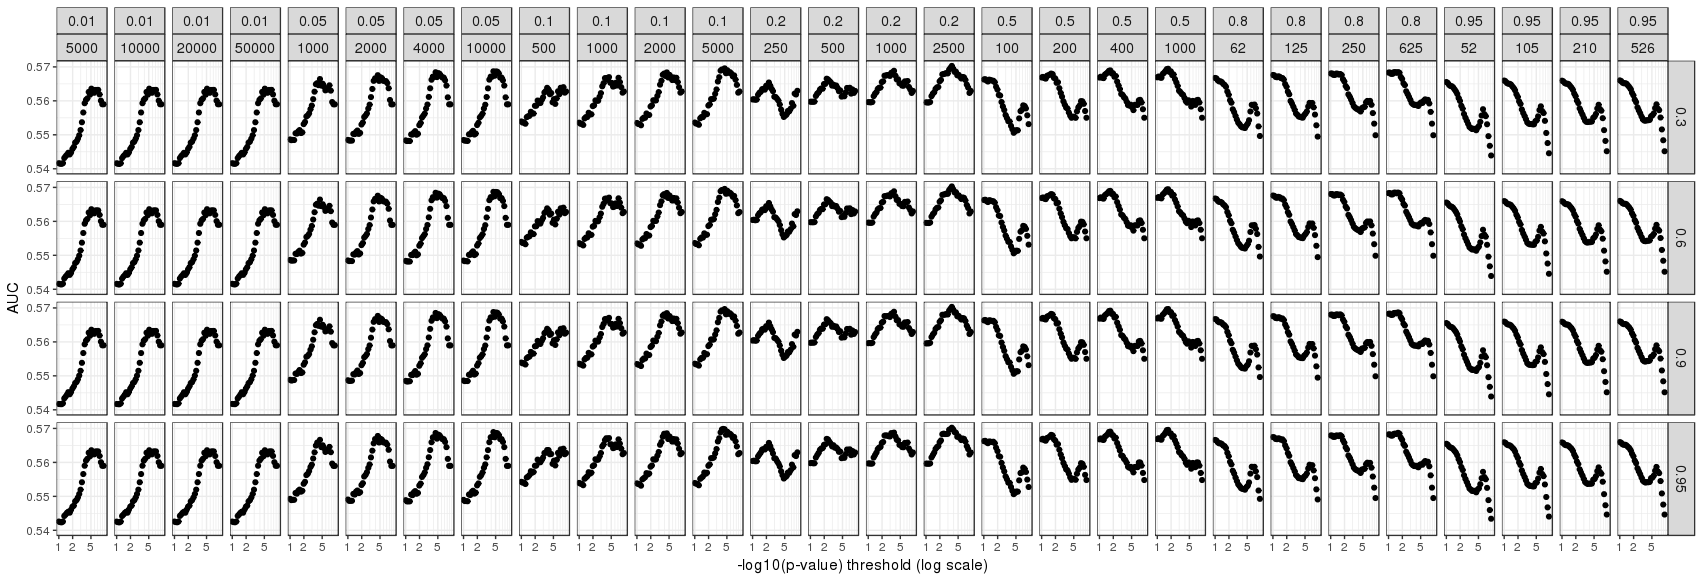
\includegraphics[width=\textwidth]{grid-asthma.png}
\caption{Asthma}
\end{subfigure}

\caption{AUC values (for the training set) when predicting disease status for many parameters of C+T in real data applications. Facets are presenting different clumping thresholds $r_{c}^2$ from 0.01 to 0.95, window sizes $w_c$ from 52 to 50,000 kb, and imputation thresholds from 0.3 to 0.95. The x-axis corresponds to the remaining hyper-parameter, the p-value threshold $p_T$; here, -log10(p-values) are represented using a logarithmic scale.}
\end{figure}

%%%%%%%%%%%%%%%%%%%%%%%%%%%%%%%%%%%%%%%%%%%%%%%%%%%%%%%%%%%%%%%%%%%%%%%%%%%%%%%%

\begin{figure}[htb]
\centerline{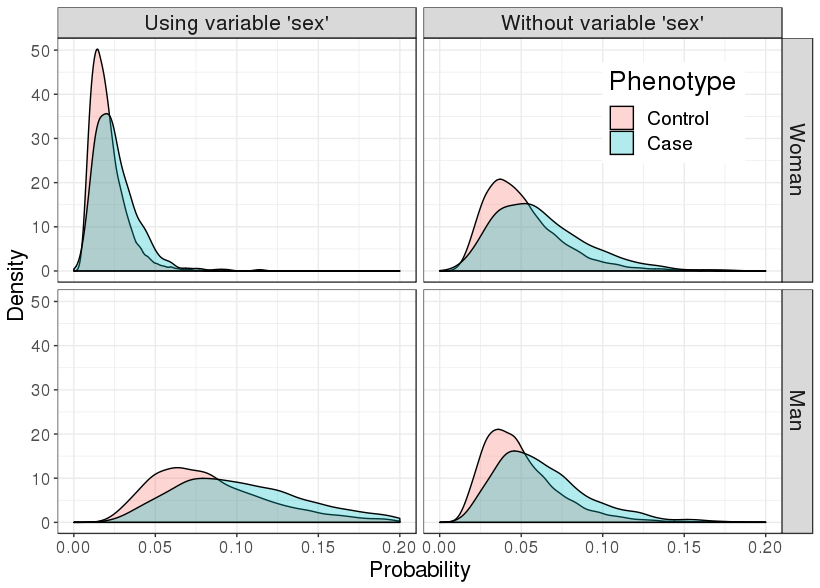
\includegraphics[width=0.8\textwidth]{dens-prob-CAD.png}}
\caption{Distribution of predicted probabilities of Coronary Artery Disease (CAD) in the UK Biobank using SCT. Upper / lower panels corresponds to women / men. Left panels correspond to a model using C+T scores and variable `sex' when fitting penalized logistic regression in the stacking step. Right panels correspond to performing stacking of C+T scores without using variable `sex'.}
\label{fig:sexCAD}
\end{figure}

\end{document}
